\documentclass[a4paper, 12pt]{article}%тип документа

%%%Библиотеки
	%\usepackage[warn]{mathtext}	
	\usepackage[T2A]{fontenc} % кодировка
	\usepackage[utf8]{inputenc} % кодировка исходного текста
	\usepackage[english,russian]{babel} % локализация и переносы
	\usepackage{caption}
	\usepackage{listings}
	\usepackage{amsmath,amsfonts,amssymb,amsthm,mathtools}
	\usepackage{wasysym}
	\usepackage{graphicx}%Вставка картинок правильная
	\usepackage{float}%"Плавающие" картинки
	\usepackage{wrapfig}%Обтекание фигур (таблиц, картинок и прочего)
	\usepackage{fancyhdr} %загрузим пакет
	\usepackage{lscape}
	\usepackage{xcolor}
	\usepackage[normalem]{ulem}
	\usepackage{hyperref}

%%%Конец библиотек




%%%Настройка ссылок
	\hypersetup
	{
		colorlinks=true,
		linkcolor=blue,
		filecolor=magenta,
		urlcolor=blue
	}
%%%Конец настройки ссылок


%%%Настройка колонтитулы
	\pagestyle{fancy}
	\fancyhead{}
	\fancyhead[L]{РТ ЛАБЫ}
	\fancyhead[R]{Талашкевич Даниил, группа Б01-009}
	\fancyfoot[C]{\thepage}
%%%конец настройки колонтитулы



							\begin{document}
						%%%%Начало документа%%%%


%%%Начало титульника
\begin{titlepage}

	\newpage
	\begin{center}
		\normalsize Московский физико-технический институт \\(госудраственный 			университет)
	\end{center}

	\vspace{6em}

	\begin{center}
		\Large Лабораторная работа по РТ лабам\\
	\end{center}

	\vspace{1em}

	\begin{center}
		\large \textbf{Безынерционные линейные цепи [24]}
	\end{center}

	\vspace{2em}

	\begin{center}
		\large Талашкевич Даниил Александрович\\
		Группа Б01-009
	\end{center}

	\vspace{\fill}

	\begin{center}
	Долгопрудный \\2021
	\end{center}
	
\end{titlepage}
%%%Конец Титульника



%%%Настройка оглавления и нумерации страниц
	\thispagestyle{empty}
	\newpage
	\tableofcontents
	\newpage
	\setcounter{page}{1}
%%%Настройка оглавления и нумерации страниц


					%%%%%%Начало работы с текстом%%%%%%
					
\section{Делитель напряжения}

\subsection{Измерение $R^{*}$}

Собрали на макетной плане делитель напряжения, с $E^{*} = 2 B$, при напряжении питания $E = 10 B$. Резистор $R_1$ выбрали $7.5 $ кОм, тогда $R_2 = 1,87 \approx 1,8$ кОм (ближайшее значение сопротивления, которые было в лаборатории на момент выполнения). При заданных $R_1, R_2$ получаем $E^{*}_{\text{теор}} = 1,94 B$. Экспериментально было получено значение $1,98$ В.

$R_l$ был выбран 1кОм, отсюда, при полученном $U_l = 0,8 B$, следует значение для $R^{*} = 1,45$ кОм.					
\subsection{Оценка коэффициента передачи $K$}

Теперь задействуем генератор, а именно подадим синусоидальное напряжение $e$. Измерив эффективные значение $u, e$ получаем значение для $K = 0,193$. Посчитаем теоретическое значение коэффициента передачи $K_{\text{теор}} = \frac{R_2}{R_1 + R_2} = 0,194$. 

\section{Параллельный сумматор}
									
\subsection{Выбираем компоненты сумматора по заданным весовым коэффициентам}

После сборки соответствующей схемы рассчитаем $R_1, R_2, R$ для того, чтобы выполнялось $\alpha = 0,4, \beta = 0,2$. Так как это система уравнений с 3-мя неизвестными 2-го ранга, то одну переменную можно выбрать 
произвольно: $R_1 = 1$ кОм $\Rightarrow R_2 = 2$ кОм, а $R = 1$ кОм. 					
					
\subsection{Проверка работы схемы}

Собираем схему, подаем на вход $E_2$ постоянное напряжение $+5 B$, а на вход $E_1$ синусоидальное с амплитудой $2 B$.

Далее, снимая показания с осциллографа, получаем значение для амплитуды переменной составляющей в сумматоре $U = \frac{0,74}{2} = 0,37 B$. Далее поочередно подав сигналы на первый и второй входы сумматора при КЗ измерим $\alpha; \beta \approx 0,42 ; 0,21$. Из полученных результатов видно, что результаты измерений совпали с теоретическими оценками.

\section{H-параметры}

\subsection{Проверка основной формулы}

Если $U_2 = 0$, то коэффициент $h_{11}$ очевиден: $h_{11} = R_1 + R_2 || R_3$. Аналогично $h_{21} = \frac{R_3}{R_2 + R_3}$ -- из закона Ома.

Если $I_1 = 0$, то $h_{12} = \frac{U_1}{U_2} = - \frac{R_3}{R_2 + R_3}$, $h_{22} = \frac{I_2}{U_2} = \frac{1}{R_2 + R_3}$ -- получается из предыдущих результатов.

\subsection{Снятие данных}

Полученные значения для $h$-параметров с помощью Micro-Cap:

\[ h_{11} = \frac{U_1}{I_1} = \frac{2,2}{10^{-3}} = 2,2 \text{кОм } (\text{при КЗ на выходе, т.е. } U_2 = 0) \]

\[ h_{21} = \frac{I_1}{I_2} = \frac{0,6 \cdot 10^{-3}}{10^{-3}} = 0,6  \text{ (при КЗ на выходе, т.е. }U_2 = 0) \]


\[ h_{22} = \frac{I_2}{U_2} = \frac{0,2 \cdot 10^{-3}}{1} = 0,2\cdot 10^{-3}  \text{ (при холостом ходе на источнике, т.е. }I_1 = 0) \]

\[ h_{22} = \frac{U_1}{U_2} = \frac{0,6}{1} = 0,6 \text{ (при холостом ходе на источнике, т.е. }I_1 = 0) \]

Проверка прямым расчетом ($R_1 = 1$ кОм, $R_2 = 2$ кОм, $R_3 = 3$ кОм) дает верные результаты $\Rightarrow$ формулы для $H$-параметров $T$-образной схемы верны.

\section{Звезда и треугольник}

\subsection{Проверка основной формулы}

Уравнение $U_1 = (R_1 + R_3)I_1 + R_3I_2$ следует из закона Ома для контура. Аналогично $U_2 = (R_2 + R_3)I_2 + R_3I_1$.

\subsection{Снятие данных}

Пересчитаем параметры звезды в параметры треугольника:

$$R_{13} = 5,5 \; \text{кОм}, R_{12} = 11/3 \; \text{кОм}, R_{23} = 11 \; \text{кОм} $$

Вычислим параметры $X_{ij}$ из схемы в программе $Micro-Cap$.

$$ X_{11} = \frac{U_1}{I_1} = \frac{4 \text{ В}}{1 \text{ мА}} = 4 \text{ кОм}$$

$$ X_{12} = \frac{U_2}{I_1} = \frac{3 \text{ В}}{1 \text{ мА}} = 3 \text{ кОм}$$

$$ X_{21} = \frac{U_2}{I_2} = \frac{3 \text{ В}}{1 \text{ мА}} = 3 \text{ кОм}$$

$$ X_{22} = \frac{U_2}{I_1} = \frac{5 \text{ В}}{1 \text{ мА}} = 5 \text{ кОм}$$

\section{Лестничные структуры}

\subsection{Исследование лестничной структуры}

Рассмотрим лестничную структуру с параметрами $\alpha = 2$, $\gamma = 1/2$, $\omega = 2$ кОм.

\begin{figure}[h!]
    \centering
    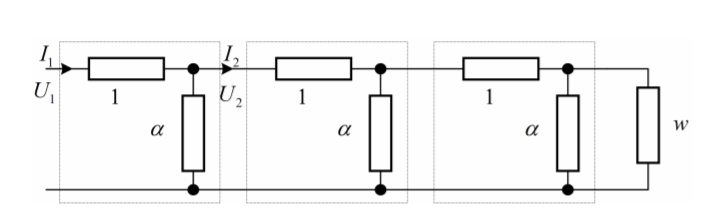
\includegraphics[width = 12 cm]{3.png}
    \caption{Лестничная структура}
    \label{fig:vac}
\end{figure}

Для напряжений и сил тока для рассматриваемой конфигурации имеем:

\begin{figure}[h!]
    \centering
    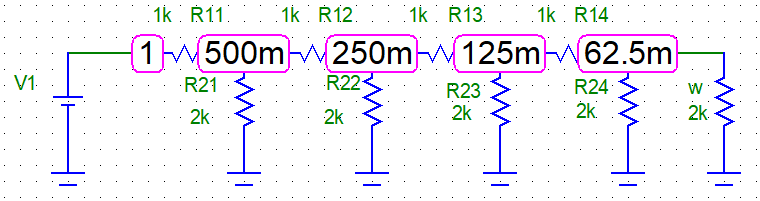
\includegraphics[width = 12 cm]{4.png}
    \caption{Напряжения лестничной структуры (1 вариант)}
    \label{fig:vac}
\end{figure}

\begin{figure}[h!]
    \centering
    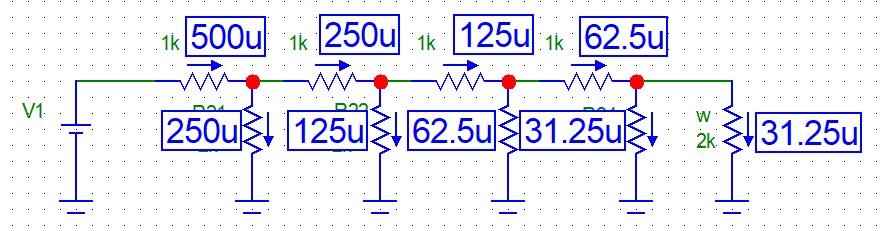
\includegraphics[width = 12 cm]{5.png}
    \caption{Силы тока лестничной структуры (1 вариант)}
    \label{fig:vac}
\end{figure}

Далее пусть $\alpha = 6$, $\gamma = 2/3$ , сопротивления $R_{2j} = 6$ кОм.

\begin{figure}[h!]
    \centering
    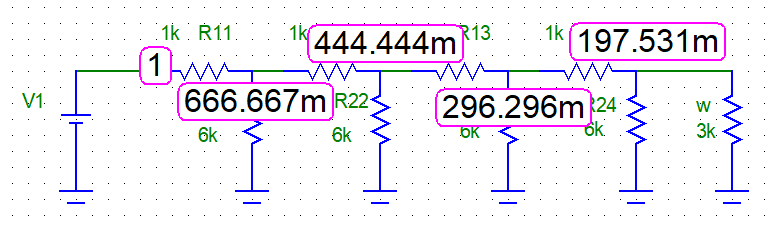
\includegraphics[width = 12 cm]{6.png}
    \caption{Напряжения лестничной структуры (2 вариант)}
    \label{fig:vac}
\end{figure}

\begin{figure}[h!]
    \centering
    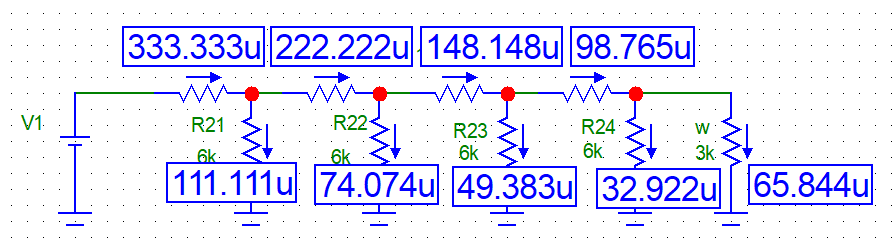
\includegraphics[width = 12 cm]{7.png}
    \caption{Силы тока лестничной структуры (2 вариант)}
    \label{fig:vac}
\end{figure}

Далее пусть $\alpha = 12$, $\gamma = 3/4$ , сопротивления $R_{2j} = 12$ кОм.

\begin{figure}[h!]
    \centering
    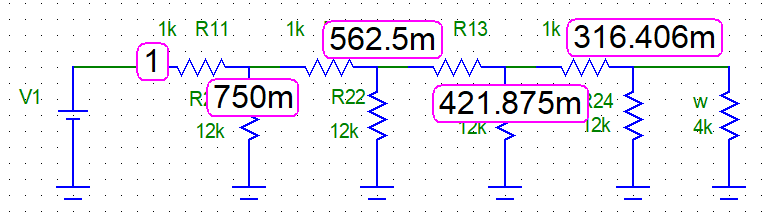
\includegraphics[width = 12 cm]{8.png}
    \caption{Напряжения лестничной структуры (3 вариант)}
    \label{fig:vac}
\end{figure}

\begin{figure}[h!]
    \centering
    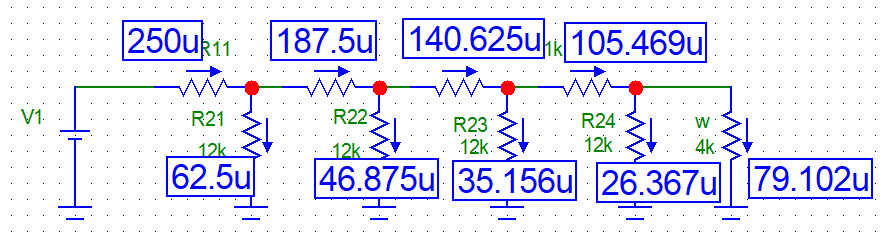
\includegraphics[width = 12 cm]{9.png}
    \caption{Силы тока лестничной структуры (3 вариант)}
    \label{fig:vac}
\end{figure}

Пусть $\alpha = 1$, $\gamma = 0.38$ , сопротивления $R_{2j} = 1$ кОм.

\begin{figure}[h!]
    \centering
    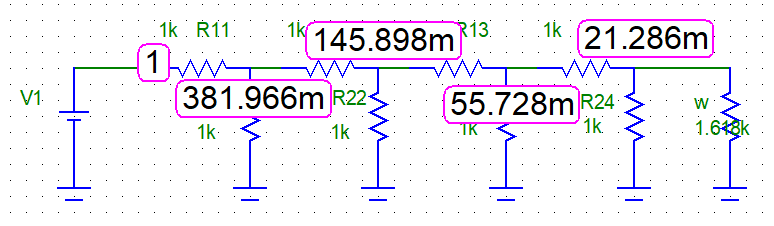
\includegraphics[width = 12 cm]{10.png}
    \caption{Напряжения лестничной структуры (4 вариант)}
    \label{fig:vac}
\end{figure}

\begin{figure}[h!]
    \centering
    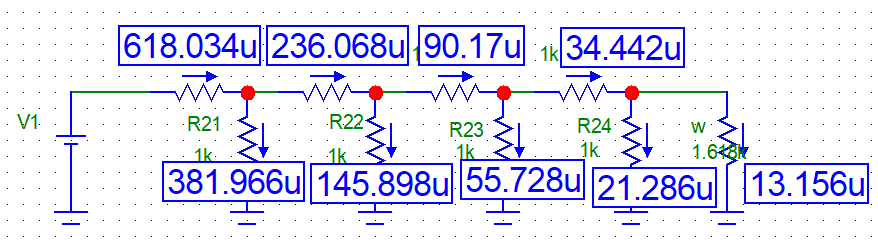
\includegraphics[width = 12 cm]{11.png}
    \caption{Силы тока лестничной структуры (4 вариант)}
    \label{fig:vac}
\end{figure}


\subsection{Исследование ЦАП}

Исследуем схему АЦП, показанную на рисунке.

\newpage

\begin{table}[h!]
\centering
\begin{tabular}{|l|l|}
\hline
Число & OUT, В \\ \hline
0001  & 1      \\ \hline
0010  & 2      \\ \hline
0011  & 3      \\ \hline
0100  & 4      \\ \hline
0101  & 5      \\ \hline
0110  & 6      \\ \hline
0111  & 7      \\ \hline
1000  & 8      \\ \hline
1001  & 9      \\ \hline
1010  & 10	   \\ \hline
1011  & 11     \\ \hline
1100  & 12     \\ \hline
1101  & 13     \\ \hline
1110  & 14     \\ \hline
1111  & 15     \\ \hline
\end{tabular}
\end{table}

\begin{figure}[h!]
    \centering
    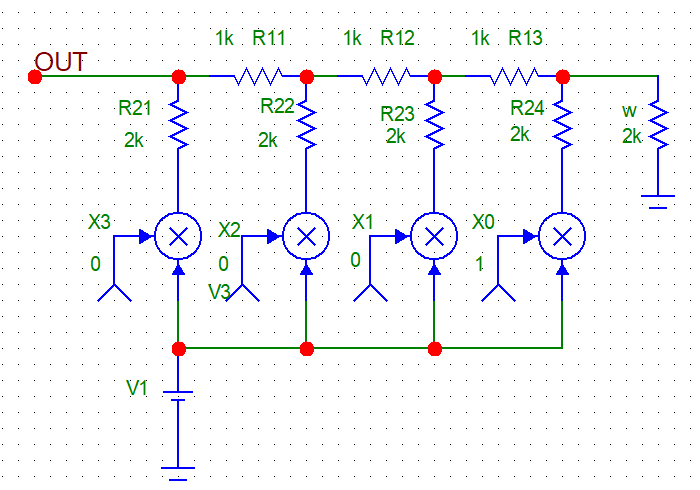
\includegraphics[width = 12 cm]{12.png}
    \caption{Схема АЦП}
    \label{fig:vac}
\end{figure}

Таблица зависимости выходящего напряжения $OUT$ в зависимости от двоичного кода $(X1,X2,X3,X4)$:













					
\end{document}